\label{chap:fund_teo}
	Este capítulo tem como objetivo apresentar a fundamentação teórica para o entendimento deste trabalho, no qual serão abordados conceitos de: Sistemas Embarcados, Modelos Formais para verificação de sistemas, Visão Computacional e Reconhecimento de Padrões.
  
    
\section{Sistemas Embarcados} 
Sistemas embarcados são sistemas baseados em microprocessadores ou microcontroladores, construídos para executar uma função ou grupos de funções programadas. Não são projetados para serem reprogramados da mesma forma que computadores pessoais \cite{heath:2002}.
%De acordo com \citeonline{heath:2002}, um sistema embarcado é um sistema baseado em um microprocessador ou microcontrolador, construído para executar uma função ou um grupo de funções programadas. Sistemas embarcados não são projetados para serem reprogramados como computadores pessoais são.
Um dos exemplos citados por \cite{heath:2002} como sistema embarcado é uma máquina de lavar, que possui vários ciclos de lavagem, painéis para acompanhar os ciclos e controle dos motores e bombas de água.
    
Já \citeonline{vahid:2002} definem sistemas embarcados como qualquer sistema que não seja um computador pessoal com as seguintes características:\begin{itemize}
\item Função única: Sistemas que são programados para um tarefa específica, que pode se repetir várias vezes.
\item Fortemente limitado: Sistema com limitações definidas nas suas métricas de projeto, como de desempenho, consumo de energia, preço e dimensões.
\end{itemize}

De acordo com \citeonline{schlett:1998}  um sistema embarcado baseado precisa executar uma tarefa específica com o menor custo energético e monetário possível. O custo energético é um dos grandes desafios encontrados no desenvolvimento de sistemas embarcados.
 

\subsection{Microcontroladores x Microprocessadores}
 Computadores modernos são baseados em microprocessadores, permitindo-os realizar várias funções, enquanto outros sistemas baseados em microcontroladores são limitados a apenas um ciclo repetido da mesma tarefa.\cite{heath:2002}
%Segundo \citeonline{white:2011} define microcontroladores como processadores com componentes atrelados a ele, com memória re-programável

Sistemas embarcados derivaram de processadores desenvolvidos para o mercado de computadores domésticos, com algumas diferenças no consumo energético, preço e componentes atrelados à \textit{CPU}. Outras diferenças são o tempo de resposta de interrupções, a quantidade de memória e portas paralelas.
\cite{schlett:1998}


\subsection{Internet das Coisas(IoT)}

A internet das coisas irá interligar todos os dispositivos atraves de sistemas embarcados, formando uma rede de dados, inteligente, ubíqua e distribuída. Os dispositivos podem trazer avanços que irão melhorar a qualidade de vida, facilitando a comunicação entre pessoas e dispositivos \cite{xia:2012}.
%\citeonline{xia:2012} afirma que a Internet das coisas irá interligar todos os dispositivos atraves de sistemas embarcados interligados por uma rede inteligente e ubíqua. 

Todos os dispositivos ao nosso redor estarão conectados a internet, isso irá resultar numa enorme quantidade de dados que terão de ser processados e apresentados sem falhas de forma eficiente. A computação em nuvem pode oferecer uma infraestrutura  de ponta a ponta, entre o dispositivo e o servidor satisfazendo essa demanda de qualquer lugar.\cite{Gubbi:2013} 

\subsection{Baixo consumo de energia}
Com o avanço da internet das coisas, uma grande demanda de dados surgiu e por sua vez a alocação e gerenciamento de dados se tornaram um problema crítico. A internet utiliza 5\% da energia gerada atualmente com a solução desses tipos de problemas, e tende a crescer cada vez mais. Em contrapartida, \textit{data centers} que utilizam fontes sustentáveis de energia terão melhor eficiência energética.\cite{Gubbi:2013} 

\section{Modelos formais para verificação de sistemas}
%falar sobre verificação de sistemas. A importância e onde é usada. Falar sobre modelos formais. Falando que a seção fala sobre exemplos de modelos formais. 
 
%\subsection{Autômatos} Não acho que seja necessário.

\subsection{Máquina finita de Estados}
TODO.


\subsection{Redes de Petri}
\todo{melhorar esse texto 12/09/17}
Redes de Petri são modelos gráficos e matemáticos que podem ser aplicados em diversos sistemas. Uma ferramenta capaz de descrever e analisar as transições do sistema, podendo ele ser concorrente, assíncrono, distribuído, paralelo e não-determinístico. O modelo gráfico é capaz de auxilar na visualização do fluxo, e a ferramenta matemática pode estruturar equações matemáticas. O comportamento de sistemas pode ser descrito em estados, um estado em uma rede de Petri é alterado de acordo com a regra de transição. \cite{murata:1989}
 
 \begin{figure}[H]
	\centering
    	\caption{\label{fig:petri}Regra de transição}
		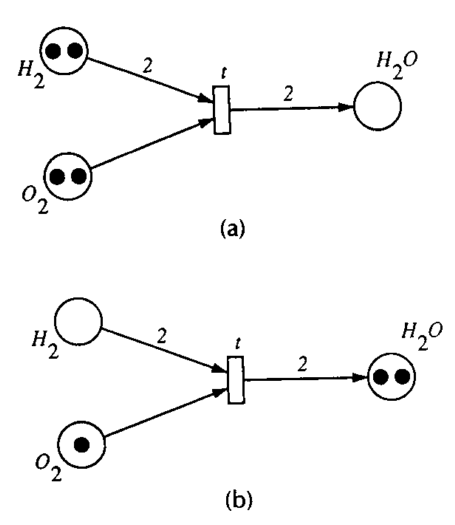
\includegraphics[width = 0.3\textwidth]	{resources/petri}
    	\legend{Regra de transição, (a) aceitação antes da transição \textbf{\textit{t}}. (b) iteração após aceitação de \textbf{\textit{t}}, \textbf{\textit{t}} está desativado.\cite{murata:1989}}
\end{figure}

\subsection{UML}
TODO.


\section{Visão Computacional}
Segundo \citeonline{marengoni:2009}, a visão computacional é uma forma de emular a visão humana, possuindo imagens como entrada, e sua saída é a interpretação dessa imagem.
Já \citeonline{bradski:2008}, definem uma parte da vasta área da visão computacional como uma transformação de dados de uma imagem em uma nova representação.

De acordo\citeonline{marengoni:2009}, o processamento da imagem geralmente é a primeira etapa do processo de visão computacional.
podendo ser dividido em três níveis: baixo-nível, nível-médio e alto-nível.
\begin{itemize}
\item Baixo-nível
	Pode ser associado a operações como redução de ruídos ou níveis de contraste da imagem.
\item Nível-médio
	São operações associadas a operações de segmentação de imagem ou reconhecimento de objetos na imagem.
\item Alto-nível
	São relacionados a tarefas de cognição associadas com a visão humana.
\end{itemize} 

\subsection{Pré-processamento de Imagem} \label{sect:preprocs}
\todo{melhorar esse texto 12/09/17}
Para evitar que imagens fiquem com interpretação limitada em determinados ambientes, por causa de diversos fatores como atenuação da luz e baixo contraste, é necessário pré-processá-las, para usar outros meios de processamento \cite{bazeille2006}. 

\subsection{Filtros para processamento digital de imagens}
TODO.

\subsubsection{Homomorphic filtering} 
	O filtro homomórfico (\textit{homomorphic filter}) é um filtro de frequência usado para corrigir iluminações não uniformes e realçar o contraste na imagem processada \cite{bazeille2006}.
     
 \begin{figure}[H]
	\centering
    	\caption{\label{fig:homofilter}Homomorphic Filtering}
		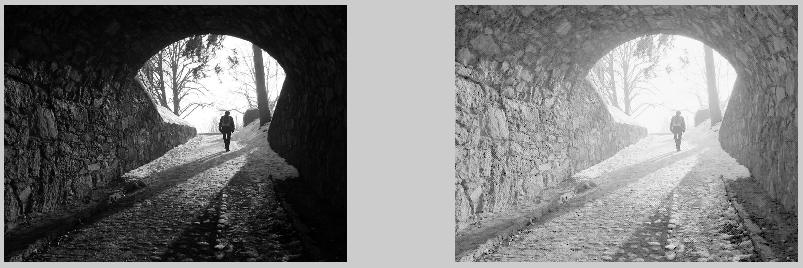
\includegraphics[width = 0.9\textwidth]	{resources/homofilter}
    	\legend{\textit{Homomorphic filtering}, usando \textit{Butterworth High Pass Filter} para fazer a filtragem \cite{mathworks:2008}}.
\end{figure}

    %Considerando o modelo de reflectância, assumimos que uma imagem é o produto descrito pela equação:
    \[
    %	f (x,y) = i(x,y).r(x,y)
    \]
    %Sendo $f(x,y)$ é a imagem captada por um sensor ótico, $i(x,y)$ o fator multiplicativo de iluminação e $r(x,y)$ a função de reflectância. 
    

\subsubsection{Anisotropic filtering}
O Filtro anisotrópico permite a simplificação de atributos da imagem para melhorar a segmentação,  suavizando as partes homogêneas preservando as bordas e melhorando-as.

 \begin{figure}[H]
	\centering
    	\caption{\label{fig:anisifilter}Anisotropic Filtering}
		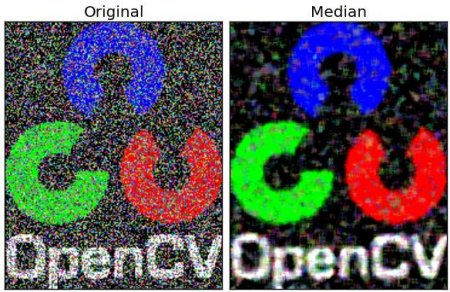
\includegraphics[width = 0.6\textwidth]	{resources/anisifilter}
    	\legend{Fonte:\cite{mathworks:2008}}.
\end{figure}

\subsection{Sensores de Aquisição de Imagens}
Segundo \citeonline{Lu:2017}, o som pode ser usado para mapear ambientes, emitindo um pulso que reflete no fundo do oceano criando um sonograma. As imagens obtidas por este sonar se assemelham a imagens óticas, com níveis de detalhes bem superiores. O reflexo criado por esse sonar tem formato de leque, com a medida que o pulso se movimenta, os reflexos irão criar séries de linhas de imagem, perpendiculares ao feixe.  

\subsection{Ferramentas para reconhecimento de images}
\todo{Definir junto ao método proposto}


\section{Reconhecimento de Padrões}

\todo{Definir junto ao método proposto}

\subsection{Aprendizado de máquina} 

\todo{Definir junto ao método proposto}

\subsection{Classificação de Padrões}




    
